\documentclass[main.tex]{subfiles}
\begin{document}
	\newpage
	\pagebreak
	\section{Vyhotovenie}
		\begin{multicols*}{2}
			\noindent Zariadenie pozostáva z plošného spoja, na ktorom sú prispájkované odpory a sloty na relé a samotné STM. Tieto sloty umožňujú jednoduchú výmenu STM a relé. Celú elektroniku chráni krabička o rozmeroch 100x81.1x55mm. Na prednej strane krabičky sa nachádzajú štyri otvory na zapojenie dvoch kanálov. Na zadnej strane krabičky sa nachádza otvor na zapojenie Micro USB a dierky na vetranie.
			
			\begin{figurehere}
				\centering
				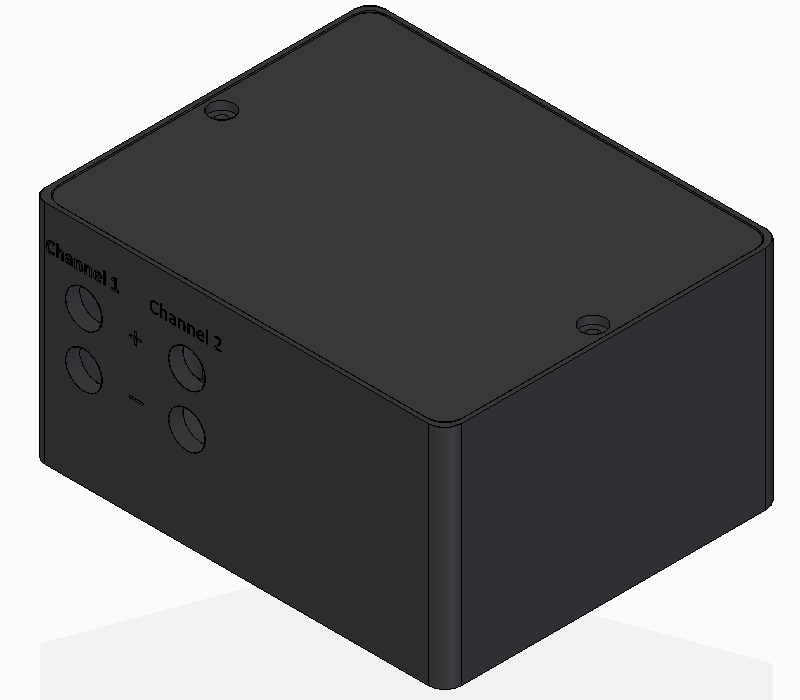
\includegraphics[width=\linewidth]{../Obrazky/Box01}
				\caption{Model krabice - predná strana}
				\label{fig:krabicaPredok}
			\end{figurehere}
			\begin{figurehere}
				\centering
				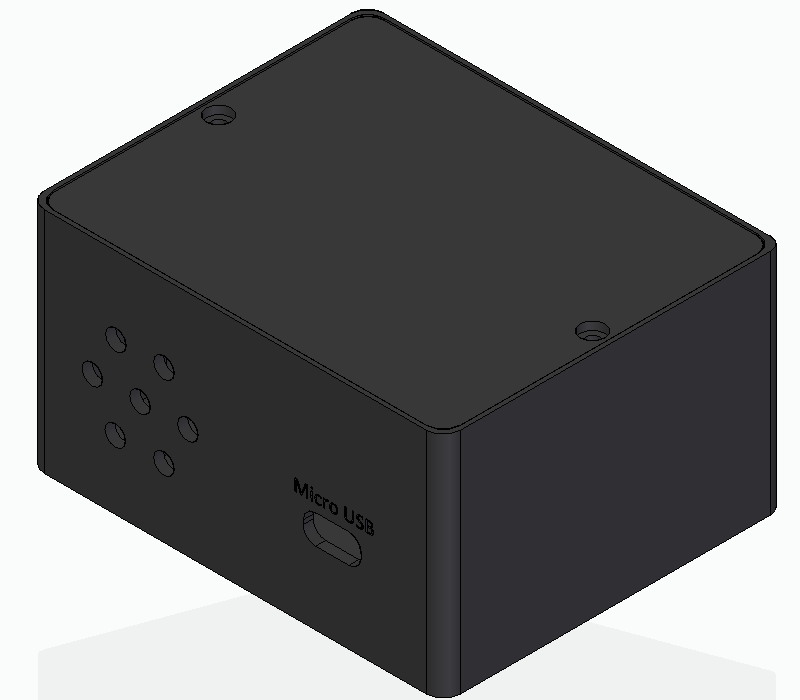
\includegraphics[width=\linewidth]{../Obrazky/Box02}
				\caption{Model krabice - zadná strana}
				\label{fig:krabicaZadok}
			\end{figurehere}
			\begin{figurehere}
				\centering
				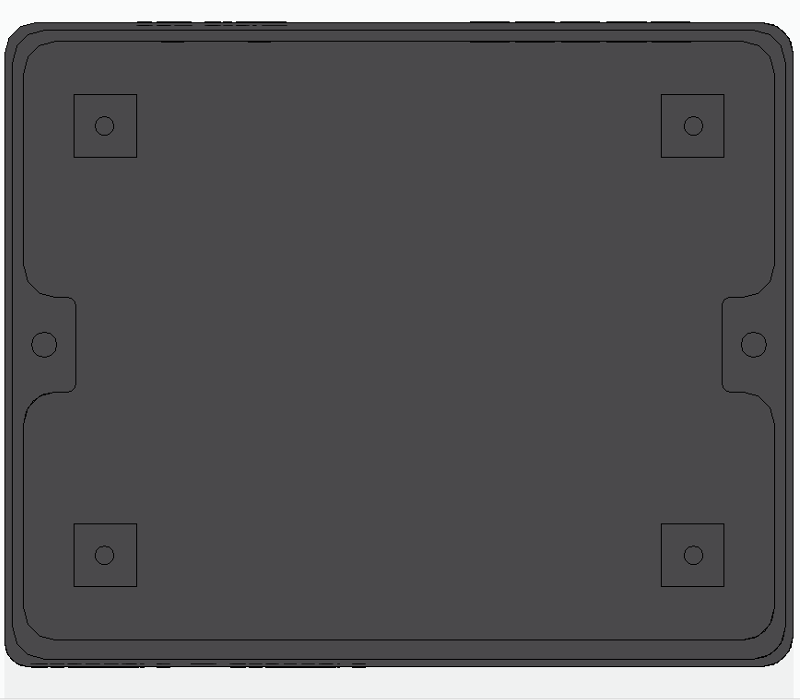
\includegraphics[width=\linewidth]{../Obrazky/Box03}
				\caption{Model krabice - zvrchu}
				\label{fig:krabicaVrch}
			\end{figurehere}
		
			\noindent Na \cref{fig:krabicaPredok}, \cref{fig:krabicaZadok} a \cref{fig:krabicaVrch} sú rôzne pohľady na model krabice. Model bol vytvorený v programe Solid Edge od Siemens.
		\end{multicols*}
\end{document}